\documentclass{article}
\usepackage{amsmath}
\usepackage[]{algorithm2e}
\usepackage{float}

\usepackage{float}
\usepackage{graphicx}


\begin{document}
\title{\textbf{FYS4150/FYS3150 - Project 2}}
\author{Ingvild Bergsbak, Oliver Hebnes and Erlend Ousdal}
\date{October 24}




\maketitle

\section{Abstract}
Mention that we choose to plot 3D

\section{Introduction}

\section{Theoretical Models and Technicalities}

\subsection{The Euler and Verlet Algorithms}

For a circular orbit around the sun, the force between the sun the the Earth is given by

$$F_G=\frac{M_Ev^2}{r}=\frac{GM_{\odot}M_E}{r^2}$$

where $M_E$ is the mass of Earth and $M_{\odot}$ is the mass of the Sun, and we have that

$$v^2r=GM_{\odot}=\frac{4\pi^2\mathrm{AU}^3}{\mathrm{yr}^2}$$

We use the average distance from the sun to the Earth, AU, as the standard length unit in this project, and for one orbit (the distance $2\pi$ AU) Earth uses one year. We insert AU $=1$ and yr $=1$ and get

$$F_G=\frac{4\pi^2\mathrm{AU}^3M_E}{r^2\mathrm{yr}^2}=\frac{4\pi^2M_E}{r^2}$$


Now we need to decompose the force. To do so we use the fact that $\sin \theta=\frac{r_y}{r}$, $\cos \theta=\frac{r_x}{r}$ and $\sin\phi=\frac{r_z}{r}$, and we get

$$F_{G,x}=\frac{4\pi^2M_E}{r^3}r_x$$
$$F_{G,y}=\frac{4\pi^2M_E}{r^3}r_y$$
$$F_{G,z}=\frac{4\pi^2M_E}{r^3}r_z$$

where $r=\sqrt{r_x^2+r_y^2+r_z^2}$.

Newton's second law gives

$$r_x''=a_x=\frac{F_G}{M_E}=\frac{4\pi^2M_E}{r^3M_E}r_x=\frac{4\pi^2}{r^3}r_x$$
$$r_y''=a_y=\frac{F_G}{M_E}=\frac{4\pi^2M_E}{r^3M_E}r_y=\frac{4\pi^2}{r^3}r_y$$
$$r_z''=a_z=\frac{F_G}{M_E}=\frac{4\pi^2M_E}{r^3M_E}r_z=\frac{4\pi^2}{r^3}r_z$$

\vskip0.5cm
The Euler method generally reads
\vskip0.5cm
\begin{algorithm}[H]
  \For{i=1,n}{
  $x_i=x_{i-1}+h\cdot x_{i-1}'$
  }
 %\caption{How to write algorithms}
\end{algorithm}
\vskip0.5cm

where $h$ is the step size.

In our case we need to calculate both the position and velocity from the acceleration, which is given by the force. This gives us the following algorithm for the $x$ direction

\vskip0.5cm
\begin{algorithm}[H]
  \For{i=1,n}{
$v_{x,i}=v_{x,i-1}-h\frac{4\pi^2}{r^3}r_{x,i-1}$\\
$r_{x,i}=r_{x,i-1}+hv_{x,i-1}$
  }
 %\caption{How to write algorithms}
\end{algorithm}
\vskip0.5cm
The acceleration becomes negative because of the directionality.

The algorithm for $y$ and $z$ direction is identical to the $x$ direction except $x$ is substituted by $y$ and $z$.

\vskip0.7cm
The general velocity Verlet method is given by
\begin{equation*}
\begin{split}
x_i&=x_{i-1}+hx_{i-1}'+\frac{h^2}{2}x_{i-1}''\\
x_i'&=x_{i-1}'+\frac{h}{2}(x_{i}''+x_{i-1}'')
\end{split}
\end{equation*}

With our values we get the following algorithm

\begin{equation*}
\begin{split}
a_{x,i-1}&=\frac{4\pi^2}{r_{i-1}^3}r_{x,i-1}\\
r_{x,i}&=r_{x,i-1}+hv_{x,i-1}+\frac{h^2}{2}a_{x,i-1}\\
a_{x,i}&=\frac{4\pi^2}{r_i^3}r_{x,i}\\
v_{x,i}&=v_{x,i-1}+\frac{h}{2}(a_{x,i}+a_{x,i-1})
\end{split}
\end{equation*}

Again, we only write the algorithm for the $x$ direction, but the $y$ and $z$ direction is completely analogous.


\subsection{The Three-Body System}

The next step towards modeling the whole solar system is to add one planet, Jupiter, to our system. The force between Earth and Jupiter is given by
$$F_{EJ}=\frac{GM_JM_E}{r_{EJ}^2}$$

where $M_J$ is the mass of Jupiter and $r_{EJ}$ is the distance between Earth and Jupiter. Decomposing the forces gives

$$F_{EJ,x}=\frac{GM_JM_E}{r_{EJ}^3}(r_{J,x}-r_{E,x})$$
$$F_{EJ,y}=\frac{GM_JM_E}{r_{EJ}^3}(r_{J,y}-r_{E,y})$$
$$F_{EJ,z}=\frac{GM_JM_E}{r_{EJ}^3}(r_{J,z}-r_{E,z})$$

The total force that works on Earth becomes

$$F_{E,x}=F_{G,x}+F_{EJ,x}=\frac{4\pi^2M_E}{r^3}r_x+\frac{GM_JM_E}{r_{EJ}^3}(r_{J,x}-r_{E,x})$$
$$F_{E,y}=F_{G,y}+F_{EJ,y}=\frac{4\pi^2M_E}{r^3}r_y+\frac{GM_JM_E}{r_{EJ}^3}(r_{J,y}-r_{E,y})$$
$$F_{E,z}=F_{G,z}+F_{EJ,z}=\frac{4\pi^2M_E}{r^3}r_z+\frac{GM_JM_E}{r_{EJ}^3}(r_{J,z}-r_{E,z})$$

and similarly for Jupiter

$$F_{J,x}=F_{GJ,x}+F_{JE,x}=\frac{4\pi^2M_J}{r^3}r_x+\frac{GM_JM_E}{r_{JE}^3}(r_{E,x}-r_{J,x})$$
$$F_{J,y}=F_{GJ,y}+F_{JE,y}=\frac{4\pi^2M_J}{r^3}r_y+\frac{GM_JM_E}{r_{JE}^3}(r_{E,y}-r_{J,y})$$
$$F_{J,z}=F_{GJ,z}+F_{JE,z}=\frac{4\pi^2M_J}{r^3}r_z+\frac{GM_JM_E}{r_{JE}^3}(r_{E,z}-r_{J,z})$$



\section{Results and Discussion}

\subsection{Earth-sun system}
It was found that the initial velocity that gives a circular orbit is $2\pi$, as given in \ref{jordensbane}.
\begin{figure}[H]
  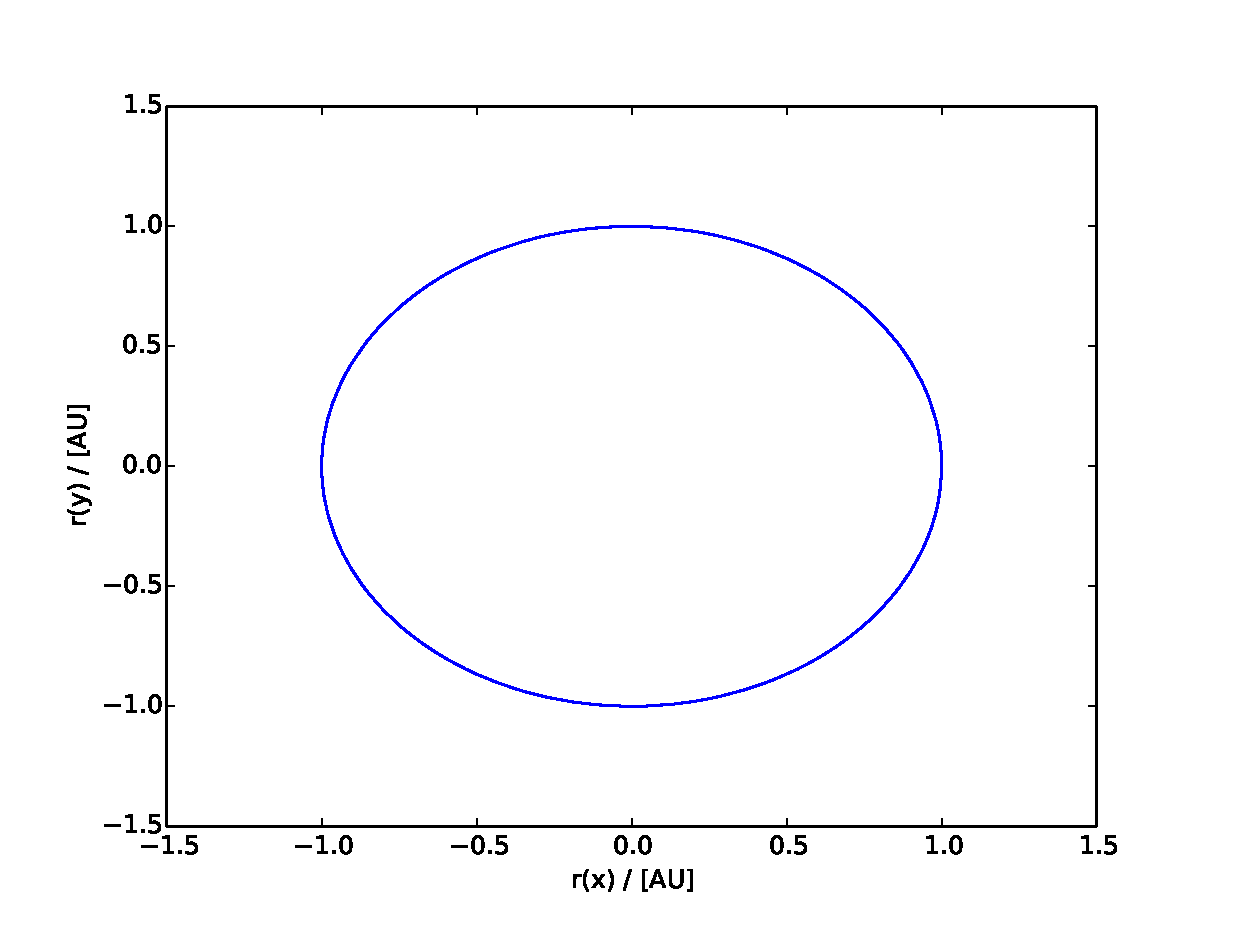
\includegraphics[scale=0.6]{3c_jordensbane_verlet_n10e6.eps}
  \caption{The Earth in a circular orbit around the origin (the sun) with intial velocity $2\pi$ in positive vertical direction. This is done by using Veilet's algorithm with $10^6$ integration points.}
  \label{jordensbane}
\end{figure}

\begin{table}[H]
    \centering
    \begin{tabular}{|l|c|c|c|r|}
    \hline
     $n$ & Verlet error  & Euler error & Time Verlet & Time Euler\\
     \hline
      $10^3$  & $1.96\cdot10^{-10}$  & $7.77\cdot10^{-2}$ & $ 4.90 (30) \cdot 10^{-3}$ & $ 4.44 (28) \cdot 10^{-3}$\\
      $10^4$  & $4.09\cdot10^{-14}$  & $7.90\cdot10^{-3}$ & $ 1.42 (27) \cdot 10^{-2}$ & $ 9.90 (40) \cdot 10^{-3}$\\
      $10^5$  & $5.22\cdot10^{-14}$  & $7.90\cdot10^{-4}$ & $ 9.81 (29) \cdot 10^{-2}$ & $ 6.42 (36) \cdot 10^{-2}$\\
      $10^6$  & $2.05\cdot10^{-13}$  & $7.89\cdot10^{-5}$ & $ 8.96 (35) \cdot 10^{-1}$ & $ 5.28 (45) \cdot 10^{-1}$\\
      \hline
    \end{tabular}
    \caption{Testing the stability and time used for Euler's algorithm and Verlet's algorithm.}
    \label{stability}
\end{table}

When comparing Euler's forward algorithm with Veilet's algorithm, it is clear that Verlet is a very accurate method compared to Euler's forward algorithm. Even if Verlet uses a bit more time than Verlet, we see that it is a small sacrifise for a much greater accuracy for our solar system.   
\section{Conclusion}


\end{document}

\begin{equation*}
\begin{split}
\end{split}
\end{equation*}
